\chapter{Machine learning}

The fundamental problem of machine learning can be formalized as follows.

\pr[]{Machine learning problem}{
    Let $X,Y$ be two sets, and $A(X,Y)$ be a set of functions from $X$ to $Y$.
    Assume moreover that we are given a subset $\mathcal F\subset A(X,Y)$ of these functions parametrized over a set $\Theta$, that is
    \begin{equation}
        \mathcal F = \left\{ \phi_\theta \in A(X,Y)\mid \theta\in \Theta \right\}.
    \end{equation}
    Then, given a function $\psi\in A(X,Y)$ the machine learning (ML) problem consists in finding $\hat \theta\in \Theta$ such that
    \begin{equation}
        \psi \approx \phi_{\hat \theta}.
    \end{equation}
    This has to be done using the \emph{available} information about $\psi$.
}

\ex[pointwise-obs]{Linear approximation and pointwise observation}{
    Let $\psi:[0,2\pi]\to \bbR$ be a continuous function (in particular, $\psi\in L^2([0,2\pi]))$).
    
    Consider $\{\phi_i\}_{i=1}^{+\infty}\subset L^2([0,2\pi])\cap C([0,2\pi])$ to be an orthonormal system for $L^2([0,2\pi])$, and for any $N\in \bbN$ let $\Theta = \bbR^N$ and consider
    \begin{equation}
        \mathcal F = \left\{ \phi_\theta = \sum_{i=1}^N \theta_i \phi_i \mid \theta_i\in \bbR^N \right\}
    \end{equation}

    Assume to be given $M$ observations $\{(x_i,y_i)\}_{i=1}^M$ such that
    \begin{equation}
        y_i = \psi(x_i), \qquad i\in \llbracket 1,M\rrbracket.
    \end{equation}
    The task here is to find $\hat \theta\in\Theta$ such that 
    \begin{equation}
        \sum_{i=1}^M \left| \phi_{\hat\theta}(x_i)-y_i \right|^2
        =\min_{\theta} 
        \sum_{i=1}^M \left| \phi_{\theta}(x_i)-y_i \right|^2.
    \end{equation}
}

\ex[]{Finite elements}{
    Let $B_1(0)\subset \bbR^d$ and $\psi : B_1(0)\to \bbR$ be a real-valued function such that $\psi\in H_0^2(B_1(0))$. 
    Then, given independent functions $\{\phi_i\}_{i=1}^N$ we can consider $\Theta=\bbR^N$ and let
    \begin{equation}
        \mathcal F = \left\{ \phi_\theta = \sum_{i=1}^N \theta_i \phi_i \mid \theta_i\in \bbR^N \right\}
    \end{equation}

    A typical situation, and the basis for the \emph{finite element methods}, is to know $f = \Delta \psi$, in which case one looks for $\hat \theta\in \Theta$ such that 
    \begin{equation}
        \|\phi_{\hat\theta}-\psi\|_{L^2} = \min_\theta \|\phi_\theta-\psi\|_{L^2}.
    \end{equation}
}

In modern machine learning one is interested in ``going beyond'' these examples, by considering a nonlinear parametrization of the approximating family $\mcF$. That is, 
\begin{center}
    the map $\theta\mapsto \phi_\theta$ is nonlinear.
\end{center}

In the following we will focus on the problem of data-fitting exoked in Example~\ref{ex:pointwise-obs}, see also Example~\ref{ex:}. This is the following.

\dfn[data-fitting-pb]{Data-fitting problem}{
    Consider the following data:
    \begin{itemize}
        \item A function $\psi:X\to Y$ to approximate, of which only a set of samples $\mfX=\{( x_i,\psi( x_i))\mid i\in \llbracket 1,M\rrbracket\}$ is known;
        \item A set $\mcF = \{\psi_\theta:X\to Y\mid \theta\in \Theta\}$ of possible approximations;
        \item A loss function $\mcL : Y\times Y \to \bbR$.
    \end{itemize}
    Then, the data-fitting problem (or minimization of the empirical risk) is the following:
    \begin{equation}
        \text{Find } \hat\theta\in\Theta \text{ such that } \hat\theta = \arg\min_{\theta} \frac1N \sum_{(x_i,\hat y_i)\in\mfX} \mcL(\phi_\theta(x_i),\hat y_i).
    \end{equation}
}

\begin{figure}
    \centering
    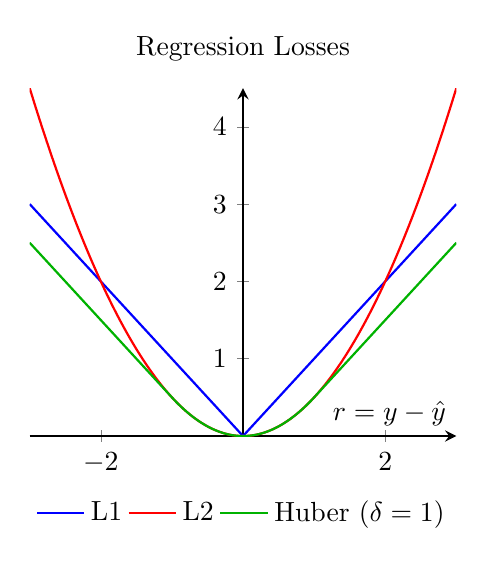
\begin{tikzpicture}
    % ---------------- Left plot: L1, L2, Huber ----------------
    \begin{axis}[
            name=regression,
            at={(0,0)}, anchor=north west,
            xlabel={$r = y - \hat{y}$},
            % ylabel={Loss},
            % grid=major,
            axis lines=middle,
            domain=-3:3,
            samples=200,
            legend style={at={(0.5,-0.15)}, anchor=north, draw=none, legend columns=3},
            width=7cm, height=6cm,
            thick,
            title={Regression Losses}
        ]
        \addplot[blue] {abs(x)};
        \addlegendentry{L1}
        \addplot[red] {0.5*x^2};
        \addlegendentry{L2}
        \addplot[green!70!black] {abs(x) < 1 ? 0.5*x^2 : 1*(abs(x)-0.5*1)};
        \addlegendentry{Huber ($\delta=1$)}
    \end{axis}
\end{tikzpicture}
% ---------------- Right plot: Cross-Entropy ----------------
\hspace{1cm}
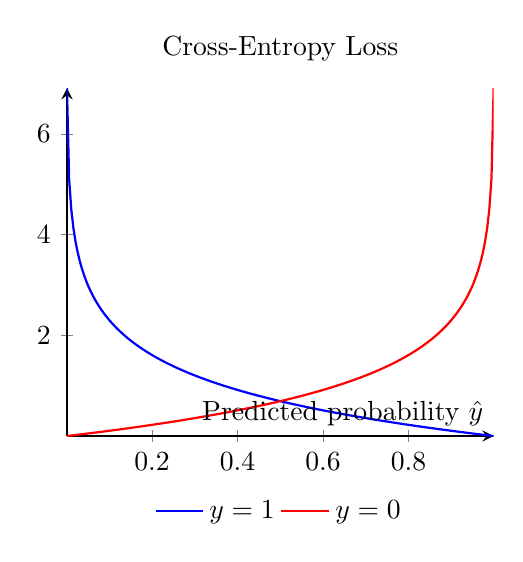
\begin{tikzpicture}
    \begin{axis}[
            xlabel={Predicted probability $\hat{y}$},
            % ylabel={Cross-Entropy Loss},
            % grid=major,
            axis lines=middle,
            domain=0.001:0.999,
            samples=200,
            width=7cm,
            height=6cm,
            thick,
            legend style={at={(0.5,-0.15)}, anchor=north, draw=none, legend columns=2},
            title={Cross-Entropy Loss}
        ]

        % y = 1
        \addplot[blue] {-ln(x)};
        \addlegendentry{$y=1$}

        % y = 0
        \addplot[red] {-ln(1-x)};
        \addlegendentry{$y=0$}
    \end{axis}
\end{tikzpicture}
    \caption{Typical loss functions for $Y=\bbR$ (right) and cross-entropy loss.}
    \label{fig:losses}
\end{figure}

When $Y$ has a vector space structure, it is natural to consider $\mcL(y,\hat y)=\ell(r)$ where $r=y-\hat y$ is called the residual.
In this case, typical choices for the loss function are appropriate norms on the space $Y$. 
% 
For example, if $Y\in \bbR^n$ one tyically considers $\mcL$ to be the $\ell_1$ or the $\ell_2$. Another common choice is the \emph{Huber error loss}, which ``mixes'' the two. It is defined for $\delta>0$ as
\begin{equation}
    \mfh_\delta(r) = 
    \begin{cases}
        \frac12 \|r\|_2^2, & \text{if }\|r\|_1\le \delta\\
        \delta\left( \|r\|_1 - \frac\delta2 \right)&\text{otherwise.}
    \end{cases}
\end{equation}
See Figure~\ref{fig:losses}, left.

A special mention need to be done in the case for \emph{classification problems}, i.e., problems where the function $\psi$ assigns a discrete label (e.g., cat or dog) to the inputs. In this the relevant values for $\psi$ are $\{0,1\}$, say, but one approximate it with functions taking value in $Y=\bbR$ and interprets values different from $0$ or $1$ as uncertain.
In this case, the most used loss function is the \emph{cross-entropy} function, which is defined by
\begin{equation}
    \mcL(y,\hat y) = -\left[ y \log \hat y + (1-y)\log(1-\hat y) \right].
\end{equation}
This function has a probabilistic interpretation and encodes, roughly speaking, the ``surprise'' of seeing $\hat y$ after the model predicted $y$.
See Figure~\ref{fig:losses}, right.









\chapter{Feed-forward neural networks}


In this chapter we introduce and discuss the simplest example of neural network\footnote{We mostly follow \cite{petersenMathematicalTheoryDeep2025}, to which we refer for further clarifications.}.
These are obtained by concatenating the simplest possible nonlinear operations:
\begin{equation}
    \phi_\theta(x) = \sigma(Wv + b), \qquad \text{where } \theta=(W,b) \in \bbR^{n\times m}\times \bbR^n.
\end{equation}
Here, the function $\sigma:\bbR\to \bbR$ is a nonlinear \emph{activation} function that is assumed to be applied element-wise to the vector $Wx+b$.
Typically activation functions are depicted in Figure~\ref{fig:activations}.

\begin{figure}[b]
    \centering
    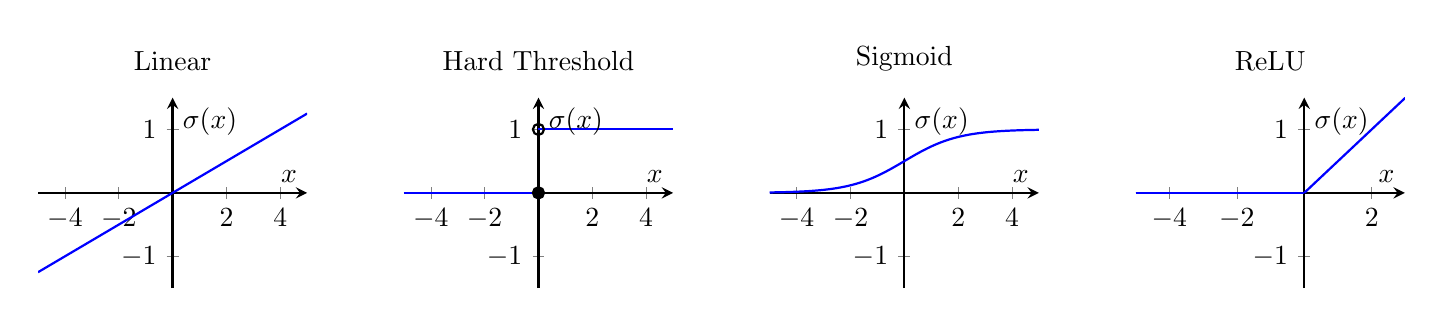
\begin{tikzpicture}[
    every axis/.style={
        width=5cm,
        height=4cm,
        % grid=major,
        axis lines=middle,
        xlabel={$x$},
        ylabel={$\sigma(x)$},
        samples=100,
        domain=-5:5,
        ymin=-1.5, ymax=1.5,
        % xtick={-4,-2,0,2,4},
        ytick={-1,0,1},
        thick
    }
]

% Arrange the four plots in a 1x2 grid
\matrix[column sep=1.2cm, row sep=1.2cm]{

% ---------- Linear ----------
\begin{axis}[title={Linear}]
    \addplot[blue] {x/4}; % scaled down for visibility
\end{axis}
&
% ---------- Hard Threshold ----------
\begin{axis}[title={Hard Threshold}]
    \addplot[blue, domain=-5:0] {0};
    \addplot[blue, domain=0:5] {1};
    \addplot[only marks, mark=*] coordinates {(0,0)};
    \addplot[only marks, mark=o, fill=white] coordinates {(0,1)};
\end{axis}
&
% ---------- Sigmoid ----------
\begin{axis}[title={Sigmoid}]
    \addplot[blue] {1/(1 + exp(-x))};
\end{axis}
&
% ---------- ReLU ----------
\begin{axis}[title={ReLU}]
    \addplot[blue, domain=-5:0] {0};
    \addplot[blue, domain=0:5] {x/2};
\end{axis}
\\
};

\end{tikzpicture}
    \caption{Activation functions}
    \label{fig:activations}
\end{figure}

\dfn[one-hidden-layer]{One-hidden layer feed-forward ANN}{
    Let $\sigma:\bbR\to \bbR$ be an activation function and let $d_1\in \bbN$.
    A scalar-valued one-hidden layer feed-forward ANN $\psi_\theta:\bbR^d\to \bbR$ is identified by the set of parameters
    \begin{equation}
        \Theta = \left\{ (W_2,b_2,W_1,b_1)\in \bbR^{1\times d_1}\times \bbR\times\bbR^{d_1\times d}\times \bbR^{d_1} \right\},
    \end{equation}
    and it reads
    \begin{equation}
        \psi_\theta(x) = W_2\, \sigma(W_1+b_1)+b_2 = \sum_{j=1}^{d_1} w_{2j} \sigma\left( \sum_{i=1}^{d} w_{ji}x_i + b_{1j} \right).
    \end{equation}

    Here, the \emph{architecture parameters} of the network are
    \begin{itemize}
        \item $d_1\in \bbN$ is the \emph{width} of the hidden layer;
        \item $W_i$ it the \emph{weight} matrix for the $i$-th layer;
        \item $b_1$ is the \emph{bias} of the \first layer.
    \end{itemize}
    }

In Figure~\ref{fig:one-hidden-layer} we present an example of a one-hidden layer feed-forward ANN

\def\layersep{4cm}
\begin{figure}[t]
    \centering
    \begin{adjustbox}{width=.7\textwidth}
        \begin{tikzpicture}[shorten >=1pt,-latex,draw=black!100, node distance=\layersep,auto]

    % INPUT LAYER
    \foreach \name / \y in {1,...,3}
    \node[input neuron] (I-\name) at (0,-2*\y+2.75) {$x_{\name}$};

    % HIDDEN LAYER
    \foreach \name / \y in {1,...,4}
    \node[hidden neuron] (H-\name) at (\layersep,-2*\y+3.5) {$x^2_\name$};

    % OUTPUT LAYER
    \node[output neuron] (O-1) at (2*\layersep,-1.25 cm) {$y$};

    % CONNECTIONS
    % Input -> Hidden
    \foreach \target in {1,...,4}
    \path (I-1) edge node[above] {$w_{1\target}$} (H-\target);

    \foreach \source in {2,...,3}
    \foreach \target in {1,...,4}
    \path[dashed] (I-\source) edge  (H-\target);

    % Hidden -> Output
    \foreach \source in {1,...,4}
    \path (H-\source) edge node[above] {$w_{\source3}$} (O-1);

    % ANNOTATIONS
    \node[annot,above of=H-1, node distance=1.5cm, align=center] (hl) {Hidden layer\\(\second layer)};
    \node[annot,above of=O-1, node distance=2.25cm, align=center] (hl2) {Output layer\\(\third layer)};
    \node[annot,left of=hl, align=center] {Input layer\\(\first layer)};

\end{tikzpicture}

% \begin{tikzpicture}[shorten >=1pt,-latex,draw=black!100, node distance=\layersep,auto]

%     \foreach \name / \y in {1,...,3}
%     \node[input neuron] (I-\name) at (0,-3*\y+2.75) {$x_{\name}$};
%     \path[yshift=1.5cm]
%     node[hidden neuron] (H-1) at (\layersep,-1 cm) {}
%     node[hidden neuron] (Q-1) at (\layersep,-2.5 cm) {}
%     node[hidden neuron] (H-2) at (\layersep,-4 cm) {}
%     node[hidden neuron] (Q-2) at (\layersep,-5.5 cm) {}
%     node[hidden neuron] (H-3) at (\layersep,-7 cm) {}
%     node[hidden neuron] (Q-3) at (\layersep,-8.5 cm) {};
%     \node[hidden neuron] (H2-1) at (2*\layersep,-3*1+2.75) {};
%     \node[hidden neuron] (H2-2) at (2*\layersep,-3*2+2.75) {};
%     \node[hidden neuron] (H2-3) at (2*\layersep,-3*3+2.75) {};
%     \node[output neuron] (H3-1) at (3*\layersep,-3.25 cm) {};
%     \node[annot,right of=H3-1, node distance=1.7cm, align=center] () {};

%     \foreach \y in {1,...,3}
%     \foreach \target in {H,Q}
%     \foreach \source in {1,...,3}
%     \path (I-\source) edge (\target-\y);
%     \foreach \y in {1,...,3}
%     \foreach \source in {H,Q}
%     \foreach \target in {1,...,3}
%     \path (\source-\y) edge (H2-\target);
%     \foreach \y in {1,...,3}
%     \path (H2-\y) edge (H3-1);


%     \node[annot,above of=H-1, node distance=1.5cm, align=center] (hl) {\first hidden layer\\(\second layer)};
%     \node[annot,above of=H2-1, node distance=2.25cm, align=center] (hl2) {\second hidden layer\\(\third layer)};
%     \node[annot,above of=H3-1, node distance=5.25cm, align=center] (hl3) {Output layer\\(\fourth layer)};
%     \node[annot,left of=hl, align=center] {Input layer\\ (\first layer)};

% \end{tikzpicture}
    \end{adjustbox}
    \caption{\label{fig:one-hidden-layer}Graphical illustration of an single hidden layer ANN, yielding a function from $\bbR^3$ to $\bbR$. We only explicited the weights relative to the first variable.}
\end{figure}

The general expression for a feed-forward ANN can then be inferred, see Figure~\ref{fig:deepANN} for a graphical representation.

\dfn[]{Feed-forward fully-connected ANN}{
    Let $\sigma:\bbR\to \bbR$ be an activation function and let $d_1,\ldots, d_L\in \bbN$.
    An $N$-hidden layer feed-forward ANN $\phi\theta:\bbR^{d_0}\to \bbR^{d_{L+1}}$ is identified by the set of parameters
    \begin{equation}
        \Theta = \left\{ (W_{L+1}, b_{L+1},\ldots,W_1,b_1) \mid W_{\ell}\in\bbR^{d_{\ell}\times d_{\ell-1}}, \, b_\ell\in \bbR^{d_\ell} \right\}.
    \end{equation}
    The corresponding function is then
    \begin{equation}
        \label{eq:ANN}
        \phi_\theta(x) = \phi^{L+1} \circ \phi^L \circ\cdots\phi^1(x),
    \end{equation}
    where 
    \begin{gather}
        \phi^{\ell}: x^{(\ell-1)} \in \bbR^{d_{\ell-1}}\mapsto x^{(\ell)}:=\sigma(W_\ell x^{(\ell-1)}+b_\ell)\in \bbR^{d_\ell}, \qquad \forall \ell\in \llbracket 1,L\rrbracket\\
        \phi^{L+1}: x^{(L)} \in \bbR^{d_{L}}\mapsto x^{(L+1)}:=W_L x^{(L)}\in \bbR^{d_{L+1}}.
    \end{gather}

    Here, the \emph{architecture parameters} of the network are
    \begin{itemize}
        \item $d_\ell\in \bbN$, $\ell\in \llbracket1,L\rrbracket$, is the \emph{width} of the \nth{$\ell$} hidden layer;
        \item $W_\ell$ it the \emph{weight} matrix for the \nth{$\ell$} layer;
        \item $b_\ell$ is the \emph{bias} of the \nth{$\ell$} layer;
        \item $x^{\ell}$ collects the output of the \emph{neurons} in the \nth{$\ell$} layer;
    \end{itemize}



    Neural networks of depth one are called \emph{shallow}, if the depth is larger than one they are called \emph{deep}. 
}

\begin{figure}
    \centering
	% \hspace{-2cm}
    \begin{adjustbox}{width=.9\textwidth}
         \begin{tikzpicture}[shorten >=0pt,-latex,draw=black!100, node distance=\layersep,auto, scale=0.92]
     \def\layersep{2.9cm}
     \def\neuronsep{1.8cm}
     \def\ninput{3}
     \def\nhidden{5}
     \def\noutput{3}
 
     \tikzmath{
         \ninputl=\ninput-1;
         \nhiddenl=\nhidden-1;
         \noutputl=\noutput-1;
         \nmax=max(\ninput,\nhidden,\noutput);
     }
 
     \foreach \inode in {1,...,\ninputl}
     \node[input neuron] (I-\inode) at (0,.5*\ninput*\neuronsep-\inode*\neuronsep+\neuronsep) {$\inode$};
     \node (I-dots) at (0,.5*\ninput*\neuronsep-\ninputl*\neuronsep) {$\vdots$};
     \node[input neuron] (I-\ninput) at (0,.5*\ninput*\neuronsep-\ninput*\neuronsep) {$l_0$};
 
     \foreach \inode in {1,...,\nhiddenl}
     \node[hidden neuron] (H1-\inode) at (\layersep,.5*\nhidden*\neuronsep-\inode*\neuronsep+\neuronsep) {$\inode$};
     \node (H1-dots) at (\layersep,.5*\nhidden*\neuronsep-\nhiddenl*\neuronsep) {$\vdots$};
     \node[hidden neuron] (H1-\nhidden) at (\layersep,.5*\nhidden*\neuronsep-\nhidden*\neuronsep) {$x_1$};
 
     \foreach \inode in {1,...,\nhiddenl}
     \node[hidden neuron] (H2-\inode) at (2*\layersep,.5*\nhidden*\neuronsep-\inode*\neuronsep+\neuronsep) {$\inode$};
     \node (H2-dots) at (2*\layersep,.5*\nhidden*\neuronsep-\nhiddenl*\neuronsep) {$\vdots$};
     \node[hidden neuron] (H2-\nhidden) at (2*\layersep,.5*\nhidden*\neuronsep-\nhidden*\neuronsep) {$x_2$};
 
     \foreach \inode in {1,...,\nhiddenl}
     \node (Hdots-\inode) at (3*\layersep,.5*\nhidden*\neuronsep-\inode*\neuronsep+\neuronsep) {$\cdots$};
     \node (Hdots-dots) at (3*\layersep,.5*\nhidden*\neuronsep-\nhiddenl*\neuronsep) {$\ddots$};
     \node (Hdots-\nhidden) at (3*\layersep,.5*\nhidden*\neuronsep-\nhidden*\neuronsep) {$\cdots$};
 
     \foreach \inode in {1,...,\nhiddenl}
     \node[hidden neuron] (H3-\inode) at (4*\layersep,.5*\nhidden*\neuronsep-\inode*\neuronsep+\neuronsep) {$\inode$};
     \node (H3-dots) at (4*\layersep,.5*\nhidden*\neuronsep-\nhiddenl*\neuronsep) {$\vdots$};
     \node[hidden neuron] (H3-\nhidden) at (4*\layersep,.5*\nhidden*\neuronsep-\nhidden*\neuronsep) {$x_{N}$};
 
     \foreach \inode in {1,...,\noutputl}
     \node[output neuron] (O-\inode) at (5*\layersep,.5*\noutput*\neuronsep-\inode*\neuronsep+\neuronsep) {$\inode$};
     \node (O-dots) at (5*\layersep,.5*\noutput*\neuronsep-\noutputl*\neuronsep) {$\vdots$};
     \node[output neuron] (O-\noutput) at (5*\layersep,.5*\noutput*\neuronsep-\noutput*\neuronsep) {$x_{N+1}$};
 
     \foreach \inode in {1,...,\ninput}
     \foreach \hnode in {1,...,\nhidden}
     \path (I-\inode) edge (H1-\hnode);
 
     \foreach \inode in {1,...,\nhidden}
     \foreach \hnode in {1,...,\nhidden}
     \path (H1-\inode) edge (H2-\hnode);
 
     \foreach \inode in {1,...,\nhidden}
     \foreach \hnode in {1,...,\nhidden}
     \path (H2-\inode) edge [-] (Hdots-\hnode);
 
     \foreach \inode in {1,...,\nhidden}
     \foreach \hnode in {1,...,\nhidden}
     \path (Hdots-\inode) edge (H3-\hnode);
 
     \foreach \inode in {1,...,\nhidden}
     \foreach \hnode in {1,...,\noutput}
     \path (H3-\inode) edge (O-\hnode);
 
     \node[annot] (input) at (0,.5*\nmax*\neuronsep+.5*\neuronsep) {Input layer\\(\first layer)};
     \node[annot] (hidden1) at (\layersep,.5*\nmax*\neuronsep+.5*\neuronsep) {\first hidden layer\\(\second layer)};
     \node[annot] (hidden2) at (2*\layersep,.5*\nmax*\neuronsep+.5*\neuronsep) {\second hidden layer\\(\third layer)};
     \node[annot] (dots) at (3*\layersep,.5*\nmax*\neuronsep+.5*\neuronsep) {$\cdots$};
     \node[annot] (hidden3) at (4*\layersep,.5*\nmax*\neuronsep+.5*\neuronsep) {\nth{$N$} hidden layer\\(\nth{$N+1$} layer)};
     \node[annot] (output) at (5*\layersep,.5*\nmax*\neuronsep+.5*\neuronsep) {Output layer\\(\nth{$(N+2)$} layer)};
 \end{tikzpicture}
    \end{adjustbox}
\caption{\label{fig:deepANN}Graphical illustration of a fully-connected feedforward ANN consisting of
$N+2\in\bbN$ affine transformations (i.e., consisting of $N+1$ layers: one input layer, $N$ hidden layers, and one output layer). Image from \cite{jentzenMathematicalIntroductionDeep2023}.}
% with $l_-1\in\bbN$ neurons on the input layer (i.e., with $l_0$-dimensional input layer), with
% $l_0\in\bbN$ neurons on the \first hidden layer (i.e., with $l_1$-dimensional \first hidden layer),
% with $l_1\in\bbN$ neurons on the \second hidden layer (i.e., with $l_2$-dimensional \second hidden layer),
% $\dots$, with $l_{L-2}$ neurons on the \nth{$(L-1)$} hidden layer (i.e., with $(l_{L-1})$-dimensional \nth{$(L-1)$} hidden layer),
% and with $l_L$ neurons in the output layer (i.e., with $l_L$-dimensional output layer). Image from \cite{jentzenMathematicalIntroductionDeep2023}.}
\end{figure}

\textbf{Remark: }
In this chapter we focus on this type of neural networks, although many adjustments are possible (as we will see in Chapter~\ref{chp:resnets}).
Some notable ones are:
\begin{itemize}
    \item The activation functions $\sigma$ can be different layer to layer, or even neuron to neuron.
    \item The output of layer $\ell$ could not only depend on layer $\ell-1$, but also on any combination of the preceding layers from $0$ to $\ell-1$ (i.e., $\phi^\ell$ can depend on $(x^{(0)},\ldots, x^{(\ell-1)})$). These are called \emph{skip connections} and the corresponding networks are \emph{residual}.
    \item Conversely, information could flow backwards, in the sense that layers $\ell-1$ to $L+1$ could serve as input for layer $\ell$. This creates loops in the flow of information, and one has to introduce a time index $t\in \bbN$, as the output of a node at time step $t$ might be different from the output at time step $t+1$. These networks are called \emph{recurrent}.
\end{itemize}


\section{Learning and backpropagation}

Once a loss function has been chosen, the data-fitting problem of Definition~\ref{def:data-fitting-pb} can be solved using the algorithms presented in Chapter~\ref{chp:numerical-algo}, along with their various extensions.
All of these algorithms, however, require the computation of the gradient of the loss function, which in turn involves differentiating the function $\phi_\theta$ from \eqref{eq:ANN}.  
This task is particularly challenging because $\phi_\theta$ is defined as a composition of many functions. Even in the simplified case where $\sigma$ is the identity (i.e., $\sigma(x) = x$), expanding \eqref{eq:ANN} explicitly leads to a sum with an order of $d_1 \times \dots \times d_N$ terms.  
In contemporary neural networks, the layer dimensions $d_1, \dots, d_N$ are so large that explicitly computing such a sum is completely infeasible, which is why efficient methods like backpropagation are essential.

\ass[]{}{
    Assume that the loss function $\mcL:\bbR^{d_{L+1}}\times \bbR^{d_{L+1}}\to \bbR$ is differentiable, and that a set $\mfX=\{(x_i,y_i) \in \bbR^{d_0}\times \bbR^{d_{L+1}}\mid i\in \llbracket 1,M\rrbracket\}$ is given.
}

Recall that our goal is to minimize the empirical risk 
\begin{equation}
    f(\theta) := \frac{1}{M}\sum_{i=1}^M \mcL(\phi_\theta(x_i),y_i),
\end{equation}
over all possible neural network parameters $\theta=(W_{L+1},b_{L+1},\ldots,W_1,b_1)$.
We thus need to find an efficient way to compute 
\begin{equation}
    \frac{\partial}{\partial b_\ell}\mcL(\phi_\theta(x),y)\in \bbR^{d_\ell}
    \qquad\text{and}\qquad
    \frac{\partial}{\partial W_\ell}\mcL(\phi_\theta(x),y)\in \bbR^{d_\ell\times d_{\ell-1}}.
\end{equation}
We have the following.

\thm[]{Backpropagation}{
    Let $x,y\in \bbR^{d_0}$ be fixed and define $\bar x^{(\ell)},\alpha^{(\ell)}\in \bbR^{d_\ell}$ by
    \begin{equation}
        \label{eq:backprop}
        \begin{cases}
        \bar x^{(1)} = W_1 x + b_1, \\
        \bar x^{(\ell)} = W_\ell \sigma(\bar x^{\ell-1})+b_\ell, \quad \ell\in \llbracket 2,L+1\rrbracket.
        \end{cases}
        \qquad
        \begin{cases}
            \alpha^{(L+1)} = \frac{\partial}{\partial \bar x^{L+1}}\mcL(\bar x^{L+1},y),\\
            \alpha^{(\ell)} = \sigma'(\bar x^{\ell})\odot (W_{\ell+1})^\top \alpha^{(\ell+1)}, \quad \ell\in \llbracket L,1\rrbracket.
        \end{cases}
    \end{equation}
    Here, we denoted by $\odot$ the elementwise product of vectors (i.e., $(v\odot w)_i=v_iw_i$).
    
    Then, it holds
    \begin{gather}
    \frac{\partial}{\partial b_\ell}\mcL(\phi_\theta(x),y) = \alpha^{(\ell)}, \qquad \ell\in \llbracket 1,L+1\rrbracket,\\
        \frac{\partial}{\partial W_1}\mcL(\phi_\theta(x),y) = \alpha^{(1)}x^\top, \qquad\text{and}\qquad 
        \frac{\partial}{\partial W_\ell}\mcL(\phi_\theta(x),y) = \alpha^{(\ell)}\sigma(\bar x^{(\ell-1)})^\top, \qquad \ell\in \llbracket 2,L+1\rrbracket.
    \end{gather}
}

\begin{remark}
    The $(\bar x^{\ell})$ defined in \eqref{eq:backprop} satisfy $x^{(\ell)}=\sigma(\bar x^{\ell})$ for $\ell\in \llbracket1,L\rrbracket$ and $x^{(L+1)}=\bar x^{(L+1)}$, where $x^{(\ell)}=\phi^\ell(x^{(\ell-1)})$ are the outputs of the neural network. 
    For this reason, $\bar x^{(\ell)}$ are called the \emph{preactivations}.
\end{remark}

\begin{remark}
    The above algorithm is called \emph{backpropagation} since it allows to compute the gradients of the loss function via the quantities $\alpha^{(\ell)}$ that are ``backpropagating'' through the network: from the last layer $L+1$ to the \first.
\end{remark}

We start by proving the following.

\lem[alpha-grad]{}{
    It holds that 
    \begin{equation}
        \alpha^{(\ell)} = \frac{\partial}{\partial \bar x^{(\ell)}}\mcL(\phi_\theta(x),y), \qquad \ell\in \llbracket1,L+1\rrbracket
    \end{equation}
}
\begin{proof}
    The statement holds for $L+1$ by definition. Assume by induction that the statement holds for $\ell+1\le L+1$ and compute by the chain rule 
    \begin{equation}
        \frac{\partial\mcL}{\partial \bar x^{(\ell)}} = 
        \left[\frac{\partial\bar x^{(\ell+1)}}{\partial \bar x^{(\ell)}} \right]^\top
        \frac{\partial\mcL}{\partial \bar x^{(\ell+1)}} = 
        \left[\frac{\partial\bar x^{(\ell+1)}}{\partial \bar x^{(\ell)}} \right]^\top
        \alpha^{(\ell+1)}.
    \end{equation} 
    The statement follows by \eqref{eq:backprop} and the direct computation
    \begin{equation}
        \left(\frac{\partial\bar x^{(\ell)}}{\partial \bar x^{(\ell+1)}}\right)_{ij} = (W_\ell)_{ij}\sigma'(\bar x^{(\ell-1)}).
    \end{equation}
\end{proof}

\begin{proof}
   We focus on proving the part concerning the derivative w.r.t.~$W_\ell$, the one w.r.t.~$b_\ell$ being similar.
   Note that $\bar x^{k}$ depends only on $(W_\ell,b_\ell)$ for $k \le \ell$. Hence, the chain rule and Lemma~\ref{th:alpha-grad} yield
   \begin{equation}
    \frac{\partial\mcL}{\partial W_\ell}=\frac{\partial\mcL}{\partial \bar x^{(\ell)}}\frac{\partial\bar x^{\ell}}{\partial W_\ell}
    =\alpha^{(\ell)}\frac{\partial\bar x^{\ell}}{\partial W_\ell}.
   \end{equation}
   The proof follows by definition of the preactivations $\bar x^{(\ell)}$. Indeed, we have
   \begin{eqnarray}
    \frac{\partial \bar x^{(1)}_k}{\partial (W_1)_{ij}} = \delta_{ki} x_j
    &\implies&
    \frac{\partial \bar x^{(1)}}{\partial W_1} = x^\top,\\
    \frac{\partial \bar x^{(\ell)}_k}{\partial (W_\ell)_{ij}} = \delta_{ki}\sigma(\bar x^{(\ell-1)}_j)
    &\implies&
    \frac{\partial \bar x^{(\ell)}}{\partial W_\ell} = \sigma(\bar x^{(\ell-1)})^\top
    , \qquad \ell\in \llbracket 2,L+1\rrbracket. 
   \end{eqnarray}
\end{proof}
    
\section{Universal approximation theorem}

In this section we are interested in providing some theoretical results justifying the use of neural networks.
More precisely, we show that (under certain assumptions) we can always find a neural network approximating a given continuous function on compact sets.
To this aim we introduce the following definitions.

\dfn[]{Universal approximator}{
    A set of functions $\mathcal H$ form $\bbR^d$ to $\bbR$ is a \emph{universal approximator} (of $C^0(\bbR^d)$) if for any $\varepsilon>0$, $K\subset\bbR^d$ compact, and $f\in C^0(\bbR^d)$, there exists $g\in \mcH$ such that 
    \begin{equation}
        \|f-g\|_K := \sup_{x\in K}|f(x)-g(x)|\le \varepsilon.
    \end{equation}
    Equivalently, $C^0(\bbR^d)$ is contained in the closure of $\mcH$ with respect to the convergence on compact sets.
}

\dfn[]{Neural network spaces}{
    Let $d,m,L,n\in \bbN$ and $\sigma:\bbR\to \bbR$. The set of all functions realized by ANNs $\phi_\theta:\bbR^d\to\bbR^m$, with at most depth $L$,  width $n$, and activation function $\sigma$ is 
    \begin{equation}
        \mcN_d^m(\sigma;L,n).
    \end{equation}
    Furthermore,
    \begin{equation}
        \mcN_d^m(\sigma;L)=\bigcup_{n\in\bbN}\mcN_d^m(\sigma;L,n).
    \end{equation}
}


\subsection{Shallow neural networks}

In this section, we establish the following result, which stresses why the nonlinear nature of the activation function is essential.

\thm[shallow-uat]{Universal approximation for shallow neural networks}{
    Let $\sigma:\bbR\to \bbR$ be an bounded piecewise continuous function\footnote{Here, we implicitly require that the discontinuity point be locally finite.}. Then, $\mcN_d^1(\sigma;1)$ is a universal approximator of $C^0(\bbR^d)$ if and only if $\sigma$ is not a polynomial.
}

\begin{remark}
    This theorem can be extended to different functional spaces and different norms.
\end{remark}

The difficult part of this theorem (which holds for more general functions \cite{leshnoMultilayerFeedforwardNetworks1993}) is to establish the universal approximation property for non-polynomial activation fucntions. The reverse implication is left as an exercice.

The result follows from the following three facts:
\begin{enumerate}
    \item If $\mcN_1^1(\sigma;1)$ is a universal approximator of $C^0(\bbR)$, then $\mcN_d^1(\sigma;1)$ is a universal approximator of $C^0(\bbR^d)$;
    \item If $\sigma\in C^\infty(\bbR)$ is not a polynomial, then $\mcN_1^1(\sigma;1)$ is a universal approximator of $C^0(\bbR)$;
    \item If $\sigma$ is bounded and piecewise continuous, functions in $\mcN_1^1(\sigma;1)$ can approximate a smooth activation function $\tilde \sigma$ which is not a polynomial.
\end{enumerate}
In particular, since $\mcN_1^1(\sigma;1)$ is a universal approximator by the second point, it follows that the same is true for $\sigma$.


Let us start by showing the first point.
An essential tool to establish universal approximation results is the Stone-Weirstrass Theorem, that we hereby recall.
\thm[]{Stone-Weierstrass}{
    Let $K\subset \bbR^d$ be compact, and $\mcH\subset C^0(K,\bbR)$ be such that
    \begin{itemize}
        \item  For all $x\in K$ there exists $f\in \mcH$ such that $f(x)\neq 0$;
        \item  For all $x,y\in K$ there exists $f\in \mcH$ such that $f(x)\neq f(y)$;
        \item $\mcH$ is an algebra of functions, i.e., $\mcH$ is closed under addition, multiplication and scalar multiplication.
    \end{itemize}
    Then, $\mcH$ is dense in $C^0(K,\bbR)$.

    In particular, this holds when $\mcH$ is the space of real-valued polynomias and $K$ is an arbitrary compact set.
}

Then, we have the following.
\lem[point1]{Point 1 of the proof of Theorem~\ref{th:shallow-uat}}{
    Assume that $\mcH$ is a universal approximator of $C^0(\bbR)$. Let $d\in \bbN$, and define  
    \begin{equation}
        \mcX = \operatorname{span}\left\{ x\mapsto g(w\cdot x) \mid w\in \bbR^d,\, g\in \mcH \right\}.
    \end{equation}
    Then, $\mcX$ is a universal approximator of $C^0(\bbR^d)$.
}

\begin{proof}
    Let us consider the space of $k$-homogeneous polynomials 
    \begin{equation}
    \bbH_k = \{ P:\bbR^d\to \bbR\mid P(x) = x^\alpha,\, \alpha\in \bbN^d_0,\, |\alpha|=k\}.
    \end{equation}
    Then, by Stone-Weierstrass Theorem, it suffices to show that $\mcX$ is a universal approximator of $\bbH_k$ for all $k$.

    Assume that this is not the case, namely that the closure $\bar\mcX$ of $\mcX$ w.r.t.~compact convergence is a proper subset of $\bbH_k$ for some $k\in \bbN$. 
    Then, by the Hahn-Banach Theorem, there exists a linear functional $\mfq\in \bbH_k'$ such that $\mfq\neq 0$ and $\ker\mfq\supset\bar\mcX$.
    Let us show that this contradicts the universal approximation property of $\mcH$.

    We start by claiming that the set $\{D^\alpha \mid |\alpha|=k\}$ is a basis for the topological dual $\bbH_k'$. Here, $D^\alpha$ is the derivative with multi-index $\alpha$, and it is immediate to check that\footnote{Recall that $\alpha!=\prod_{i=1}^d \alpha_j!$.} $D^\alpha x^\beta = \delta_{\alpha,\beta}\alpha!$ for any $|\alpha|=|\beta|=k$. Since $p(x)=x^\beta$ for $|\beta|=k$ is a basis of $\bbH_k$, this proves the claim.

    Consider now the $k$-homogeneous polynomial $p_w(x)=(w\cdot x)^k$ with $w\in \bbR^d$, and observe that it holds
    \begin{equation}
        \label{eq:multinomial}
        p_w(x) = \left[ \sum_{i=1}^d w_ix_i \right]^k = \sum_{|\alpha|=k}\frac{k!}{\alpha!}w^\alpha x^\alpha.
    \end{equation}
    By the universal approximation property of $\mcH$ we have that $p_w\in \bar\mcX$ for any $w\in \bbR^d$.
    On the other hand, by the previous claim, we have that $\mfq = \sum_{|\alpha|=k} q^\alpha D^\alpha$ for some $q^\alpha\in \bbR$, and thus by \eqref{eq:multinomial} we get
    \begin{equation}
        0=\mfq(p_w) = k! \sum_{|\alpha|=k}q^\alpha w^\alpha, \qquad \forall w\in \bbR^d \implies \mfq =0.
    \end{equation}
    We have thus reached the desired contradiction.
\end{proof}

\lem[]{Point 2 of the proof of Theorem~\ref{th:shallow-uat}}{
    If $\sigma\in C^\infty(\bbR)$ is not a polynomial, then $\mcN_1^1(\sigma;1)$ is a universal approximator for $C^0(\bbR)$.
}

\begin{proof}
    Let $\mcX=\mcN_1^1(\sigma;1)$. We proceed as in the proof of Lemma~\ref{th:point1} and show that $\mcX$ is a universal approximator for the space of polynomials. This completes the proof by the Stone-Weierstrass Theorem.

    Let $b\in \bbR$, and consider the function 
    \begin{equation}
        f_b(x,w):=\sigma(wx+b), \qquad x,w\in \bbR.
    \end{equation}
    Denoting $\partial_w^k$ the \nth{$k$} derivative w.r.t.~the variable $w$, we have that 
    \begin{equation}
        \partial^k_w f_b(x,w)=x^k\sigma^{(k)}(wx+b)
        \implies
         \partial^k_w f_b(x,w)=x^k\sigma^{(k)}(b).
    \end{equation}
    Since $\sigma\in C^\infty(\bbR)$ is not a polynomial, for any $k$ there exsists $b_k\in \bbR$ such that $\sigma^{(k)}(b_k)\neq 0$. 
    Thus, to prove the statement it suffices to show that $\partial_w^k f_{b}(\cdot,0)\in \mcX$ for any $b$. 

    To this aim, consider the function $\phi_\theta\in \mcX$ given by  
    \begin{equation}
        \phi_{\theta}(x) = \frac{1}{h} \sigma((w+h)x + b) - \frac{1}{h}\sigma(wx+b).
    \end{equation}
    This is a one-hidde layer feed-forward ANN as per Definition~\ref{def:one-hidden-layer} for the choice $d=1$, $d_1 = 2$ and 
    \begin{equation}
        W_1 = \begin{pmatrix}
            w \\ w
        \end{pmatrix},
        \qquad b_1 = \begin{pmatrix}
            b \\ b
        \end{pmatrix},
        \qquad W_2=\begin{pmatrix}
            \frac{1}{h} & \frac{1}{h}
        \end{pmatrix},
        \qquad b_2 = 0.
    \end{equation}
    A simple Taylor development in $w$ shows that for any $h>0$ there exists $\xi\in [w,w+h]$ such that
    \begin{equation}
        \phi_\theta(x) 
        = \partial_w f_b(x,w)+ \frac{h}{2}\partial_w^2 f_b(x,\xi)
        = \partial_w f_b(x,w)+\frac{h}{2}x^2\sigma''(\xi x+b).
    \end{equation}
    But $\sigma''$ is continous, and thus for any compact set $K\subset \bbR$ we have 
    \begin{equation}
        \sup_{x\in K} \sup_{|h|<1}|x^2\sigma''(\xi x+b)| \le 
        \sup_{x\in K} \sup_{|\eta-w|<1}|x^2\sigma''(\eta x+b)| <+\infty. 
    \end{equation}
    In particular, letting $h\to 0$ we see that $\phi_\theta$ converges uniformly on $K$ to $\partial_w f_b(\cdot,w)$. Thus, $\partial_w f_b(\cdot,w)\in \mcX$.
    Applying the argument inductively, shows that $\partial_w^kf_b(\cdot,w)\in \mcX$, completing the proof.
\end{proof}

To conclude the proof, we need to recall the following concept.
\dfn[]{Convolution}{
    Let $f,g\in L^\infty(\bbR)$ and assume that $g$ has compact support. Then the \emph{convolution} of $f$ and $g$ is defined as
    \begin{equation}
        f\star g(x) := \int_\bbR f(x-y)g(y)\, dy.
    \end{equation}
}

\lem[]{Point 3 of the proof of Theorem~\ref{th:shallow-uat}}{
    Assume that $\sigma:\bbR\to \bbR$ is bounded and piecewise continous. Then, for any $\varphi\in C^\infty_c$ we have that $\sigma\star\varphi\in C^\infty_c(\bbR)$ is in the closure of $\mcN_1^1(\sigma;1)$ w.r.t.~uniform convergence on compact sets.

    Moreover, if $\sigma\star \varphi$ is a polynomial for any $\varphi\in C^\infty_c(\bbR)$, then $\sigma$ is a polynomial.
}

\begin{proof}
    The fact that $\sigma\star\varphi\in C^\infty_c(\bbR)$ is standard, and follows observing that $(\sigma\star \varphi)'=\sigma\star (\varphi')$.
    For the proof of the last part of the statement, we refer to \cite[Lemma~3.15]{petersenMathematicalTheoryDeep2025}.

    Let us build an explicit sequence $f_n\in \mcN_1^1(\sigma;1)$ such that $f_n\rightarrow \sigma\star\varphi$ uniformly on compact sets. 
    Let $a>0$ be such that $\operatorname{supp}\varphi\subset[-a,a]$.  
    Then, for any $n\in \bbN$ we let $y_j=-a+2a/n$ and set
    \begin{equation}
        f_n(x) := \frac{1}N \sum_{j=0}^{N-1} \sigma(x-y_j)\varphi(y_j).
    \end{equation}
    It follows easily that $f_n\in \mcN_1^1(\sigma;1)$. Let us show the required convengerce on an arbitrary compact set $[-b,b]$, $b>0$.
    
    Since $y_{j+1}-y_j\le 1/n$, for any $x\in [-b,b]$ we have 
    \begin{equation}
        \label{eq:stima1}
        |\sigma\star \varphi(x)-f_n(x)| \le
        \sum_{j=0}^{N-1} \left| \int_{y_j}^{y_{j+1}} \left( \sigma(x-y)\varphi(y)-\sigma(x-y_j)\varphi(y_j)\right)\, dy \right|.
    \end{equation}
    Let us bound each term in the sum above. 
    
    Observe that there exists $C>0$ such that 
    \begin{equation}
        \left| \sigma(x-y)\varphi(y)-\sigma(x-y_j)\varphi(y_j)\right|
        \le C, \qquad \forall x,y\in \bbR, \, j\in \llbracket0,n-1\rrbracket.
    \end{equation}
    Then, for any $j\in \llbracket0,N-1\rrbracket$ we can estimate 
    \begin{equation}
        \label{eq:stima2}
        \left| \int_{y_j}^{y_{j+1}} \left( \sigma(x-y)\varphi(y)-\sigma(x-y_j)\varphi(y_j)\right)\, dy \right|
        \le C (y_{j+1}-y_{j}) \le \frac{C}{n}.
    \end{equation} 
    Recall that, by assumption, there exists $\{z_1,\ldots z_M\}\subset [-a,a]$ such that $\sigma$ is continous on $[-a,a]\setminus\{z_1,\ldots,z_M\}$. 
    We will use the above estimate for the at most $M$ intervals containing one of the points $x-z_i$, $i\in \llbracket1,M\rrbracket$.
    Let $J_d$ be the set of such indexes and $J_c=\llbracket0,N-1\rrbracket\setminus J_d$.
    
    Let us now fix $\varepsilon>0$ and such that $\varepsilon\le \min \{ \frac{|(x-z_i)-y_j|}2 \mid i\in \llbracket1,M\rrbracket \text{ and } j\in \llbracket0,n\rrbracket \}$ and consider the compact set
    \begin{equation}
        K = [-a,a] \setminus \bigcup_{i=1}^m (z_i-\varepsilon,z_i+\varepsilon)\supset \bigcup_{j\in J_c} [y_j,y_{j+1}].
    \end{equation}
    Observe that $\sigma$ is uniformly continuous on $K$.
    Then, for any $j\in J_c$ and $y\in [y_j,y_{j+1}]$ we have that $x-y\in K$ and $x-y_j\in K$. 
    Thus,
    \begin{equation}
        \left| \sigma(x-y)\varphi(y)-\sigma(x-y_j)\varphi(y_j)\right|
        \le |\sigma(x-y)-\sigma(x-y_j)|\,|\varphi(y)|+|\sigma(x-y_j)|\,|\varphi(y)-\varphi(y_j)| 
        \le \|\varphi\|_\infty \max_{\substack{s_1,s_2\in K\\|s_1-s_2|\le \frac{2a}n}}|\sigma(s_1)-\sigma(s_2)|
        + \|sigma\|_\infty \max_{\substack{s_1,s_2\in [-a,a]\\|s_1-s_2|\le \frac{2a}n}}|\varphi(s_1)-\varphi(s_2)| := \eta_n.
    \end{equation}
    By uniform continuity of $\sigma$ on $K$ and of $\varphi$ on $[-a,a]$ we have $\eta_n(x)\rightarrow 0$ as $n\to 0$ uniformly for $x\in [-b,b]$.
    Using  \eqref{eq:stima1} and \eqref{eq:stima2}, this shows that
    \begin{equation}
        |\sigma\star \varphi(x)-f_n(x)| \le 
        \sum_{j\in J_d} \frac Cn + \sum_{j\in J_c} \frac{\eta_n(x)}{n} \le \frac{CM}n + \eta_n(x) \rightarrow 0,
    \end{equation}
    uniformly for $x\in [-b,b]$.
\end{proof}

Putting together the above results, we complete the proof of Theorem~\ref{th:shallow-uat}.

\subsection{Deep neural networks}

As a corollary to Theorem~\ref{th:shallow-uat} we have the following.

\cor[deep-uat]{Universal approximation for deep neural netowrks}{
    Let $\sigma:\bbR\to \bbR$ be an bounded piecewise continuous function. Then, for any $L\in \bbN$, $\mcN_d^1(\sigma;L)$ is a universal approximator of $C^0(\bbR^d)$ if and only if $\sigma$ is not a polynomial.
}

The proof reduces to show that it is possible to approximate the identity with a deep network with $L-1$ layers. This is contained in the following.

\prop[deep-identity]{}{
    Let $\sigma:\bbR\to \bbR$ be differentiable and non constant on an open set.
    The, for any $L\in \bbN$ and $\varepsilon>0$, there exists a neural network $\phi\in \mcN_d^1(\sigma;L,d)$ such that 
    \begin{equation}
        |\phi(x)-x|\le \varepsilon, \qquad  \forall x\in K.
    \end{equation}
}

\begin{proof}
   We prove the statement for $L=1$, the extension to $L>1$ being straightforward.
   Let $s^\star\in \bbR$ be such that $\sigma$ is differentiable in a neighborhood of $s^\star$ and $\varsigma:=\sigma'(s^\star)\neq 0$.
    Let $b=(s^\star,\ldots,s^\star)\in \bbR^d$ and, for $\lambda>0$, define 
    \begin{equation}
        \phi_\lambda(x) := \frac{\lambda}{\varsigma} \sigma\left(\frac{x}{\lambda} + b \right) - \frac{\lambda}{\varsigma}\sigma(b).
    \end{equation}
    It is clear that $\phi_\lambda\in \mcN_d^1(\sigma;1,d)$.
    Moreover, a Taylor development easily shows that
    \begin{equation}
        \phi_\lambda(x)-x = \lambda \frac{\sigma(x/\lambda +b)-\sigma(b)}{\varsigma} - x \rightarrow 0, \qquad \text{as }\lambda\to +\infty.
    \end{equation}
    This completes the proof.
\end{proof}


\noindent\textbf{\em Proof of Corollary~\ref{th:deep-uat}:}
    We already know that $\mcN_d^1(\sigma;1)$ is an universal approximator. That is, for any $f\in C(\bbR^d)$, for any $K$ compact and any $\varepsilon>0$ there exists a shallow netowrk $\phi_1\in \mcN_d^1(\sigma;1)$ such that 
    \begin{equation}
        \| f - \phi_1\|_K \le \frac\varepsilon2.
    \end{equation}
    Concatenanting this with the deep network approximating the identity given by Proposition~\ref{prop:deep-identity} completes the proof.
\qed

\subsection{Further results}

We conclude this chapter by mentioning the following remarkable result stating that, for an appropriate activation function, it is possible to approximate every function $f\in C(K)$, where $K\subset \bbR^d$, at every accuracy $\varepsilon>0$ with a neural network of size $O(d^2)$. Remarkably, this size is independent of $f$, of $K$, and even of $\varepsilon$.
We refer to \cite[Section~3.2]{petersenMathematicalTheoryDeep2025} for a proof, based on the Kolmogorov's superposition theorem.

\thm[]{Universal approximation via superexpressive activations}{
    There exists a continuous activation function $\sigma:\bbR\to \bbR$ such that for every compact $K\subset\bbR^d$, every $\varepsilon>0$, and every $f\in C(K)$, there exists\footnote{That is, $\operatorname{width}\phi = 2d^2+2$ and $\operatorname{depth}\phi=2$} $\phi\in \mcN_d^1(\sigma; 2,2d^2+d)$ such that
    \begin{equation}
        |f(x)-\phi(x)|\le \varepsilon, \qquad \forall x\in K.
    \end{equation}
}

\chapter{Residual neural networks, neural ODEs and control}
\label{chp:resnets}